\section{Distinguish Devices}
IoT applications utilise a great variation of devices, with each having different processing power. This implies that the processing time of some specific packets can be exploited as a hint to the model of device. 

PING is therefore an ideal feature supported in 6LoWPAN that can be exploited to perform such an attack due to:
\begin{enumerate}
	\item PING is processed in a standardised routine where nearly no computation is required, minimising the noise in the data.
	\item The support of PING is required by the standard\cite{rfc4443}, making the attack universally applicable.
\end{enumerate}

\subsection{Contiki MAC}\label{TimingWithContikiMAC}
Contiki adopts a Radio Duty Cycle (RDC) protocol called Contiki MAC\cite{ContikiMAC} to preserve energy. Briefly speaking, Contiki MAC works by switching off the radio for most of the times but periodically wakes up for a short period for signal detection, and keeps the radio up only if a signal is detected. On the other hand, the sender repeats the signal when sending a packet, until a receiver acknowledges the sender or time out.

As a result, duplicated packets may be observed in the captured traffic. To best approximate the processing time for a specific PING request, the response time is defined as the timing difference between the last PING request being sent and the first PING response being replied.

\subsection{Pinging Different Devices}
We measured the PING response time for two devices, namely TelosB\cite{TelosB} and CC2538\cite{CC2538}. Optionally for TelosB, the default software AES implementation can be replaced a hardware coprocessor. The PING response time for the above platforms are shown in \Cref{PINGTiming}.

\begin{figure}[ht!]
	\centering
	\begin{subfigure}{0.4\textwidth}
	{
		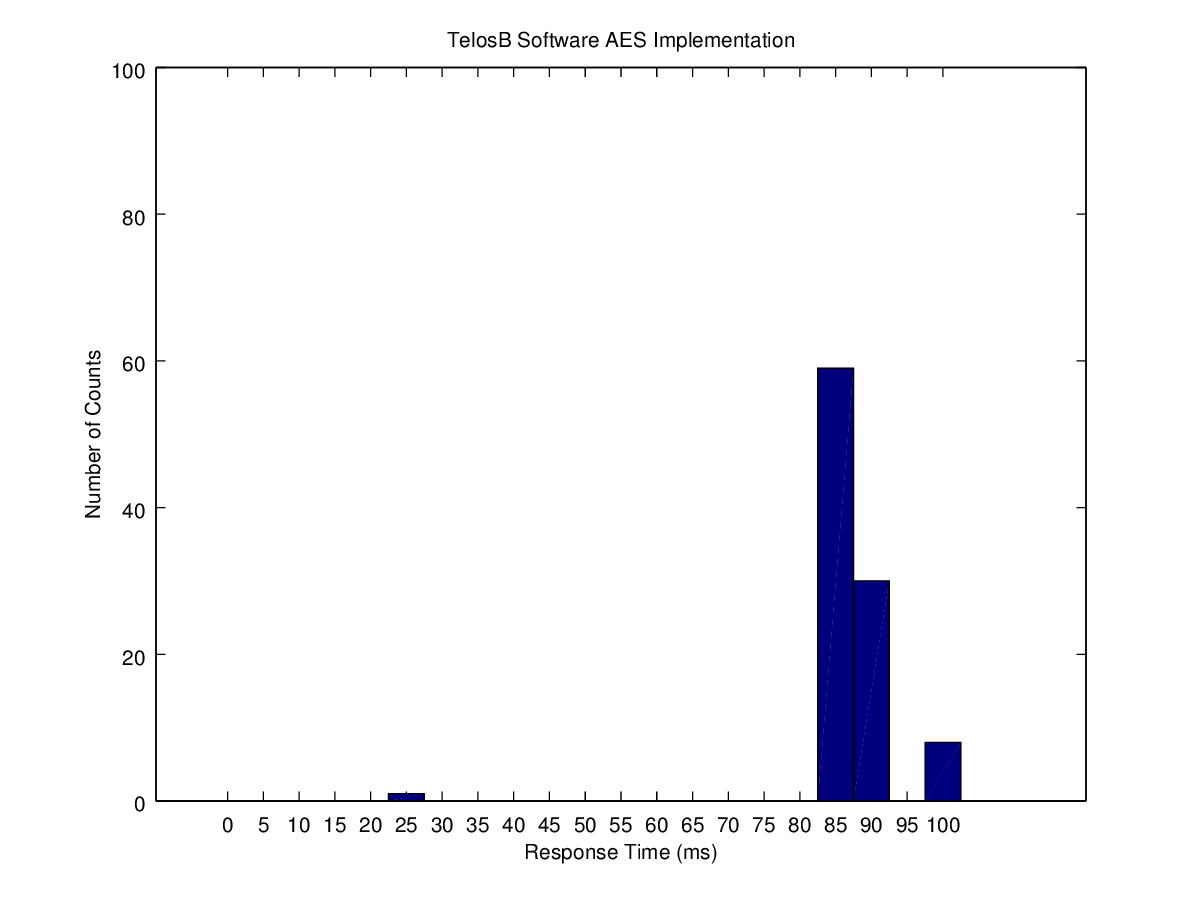
\includegraphics[width=\textwidth]{fig/noncoresec_ping_telosb_sw.png}
	}
	\end{subfigure}
	\begin{subfigure}{0.4\textwidth}
	{
		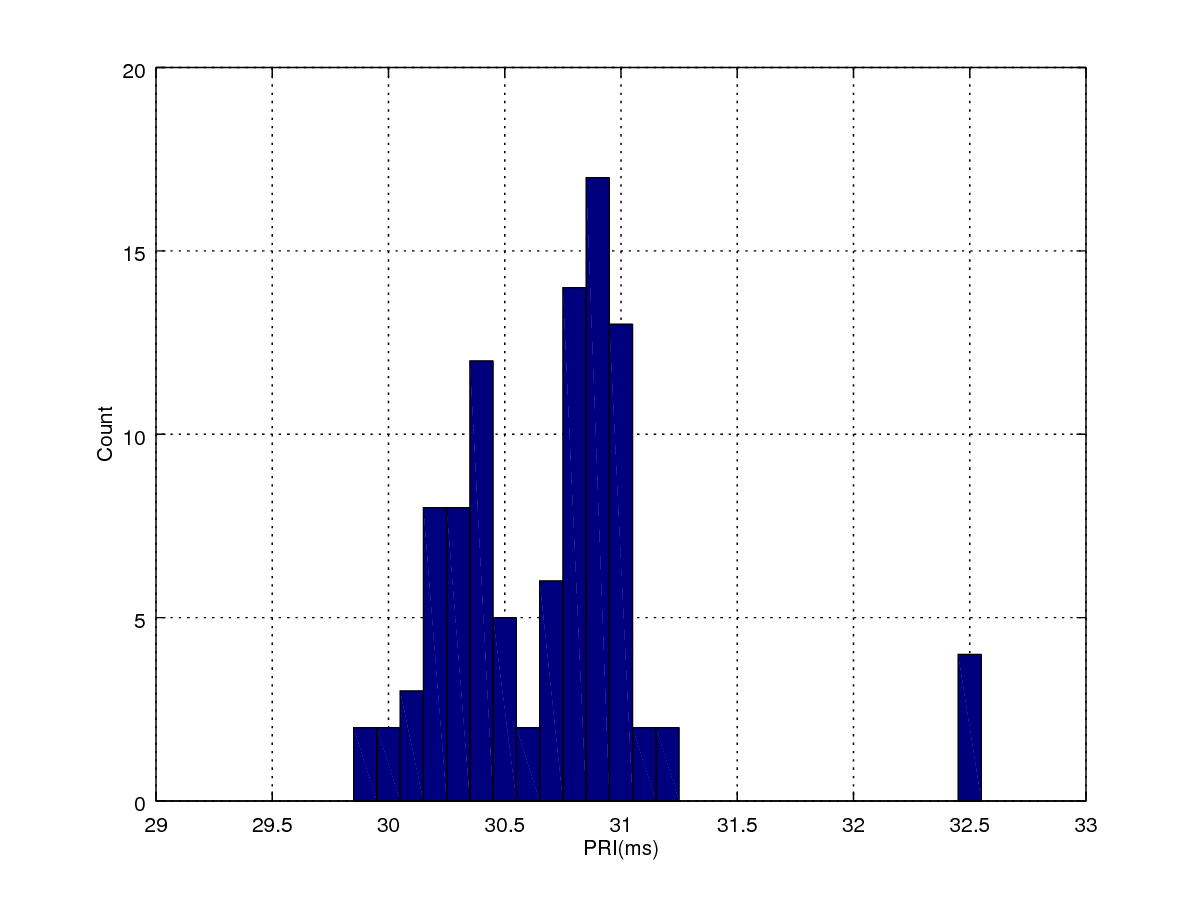
\includegraphics[width=\textwidth]{fig/noncoresec_ping_telosb_hw.png}
	}
	\end{subfigure}
	\begin{subfigure}{0.4\textwidth}
	{
		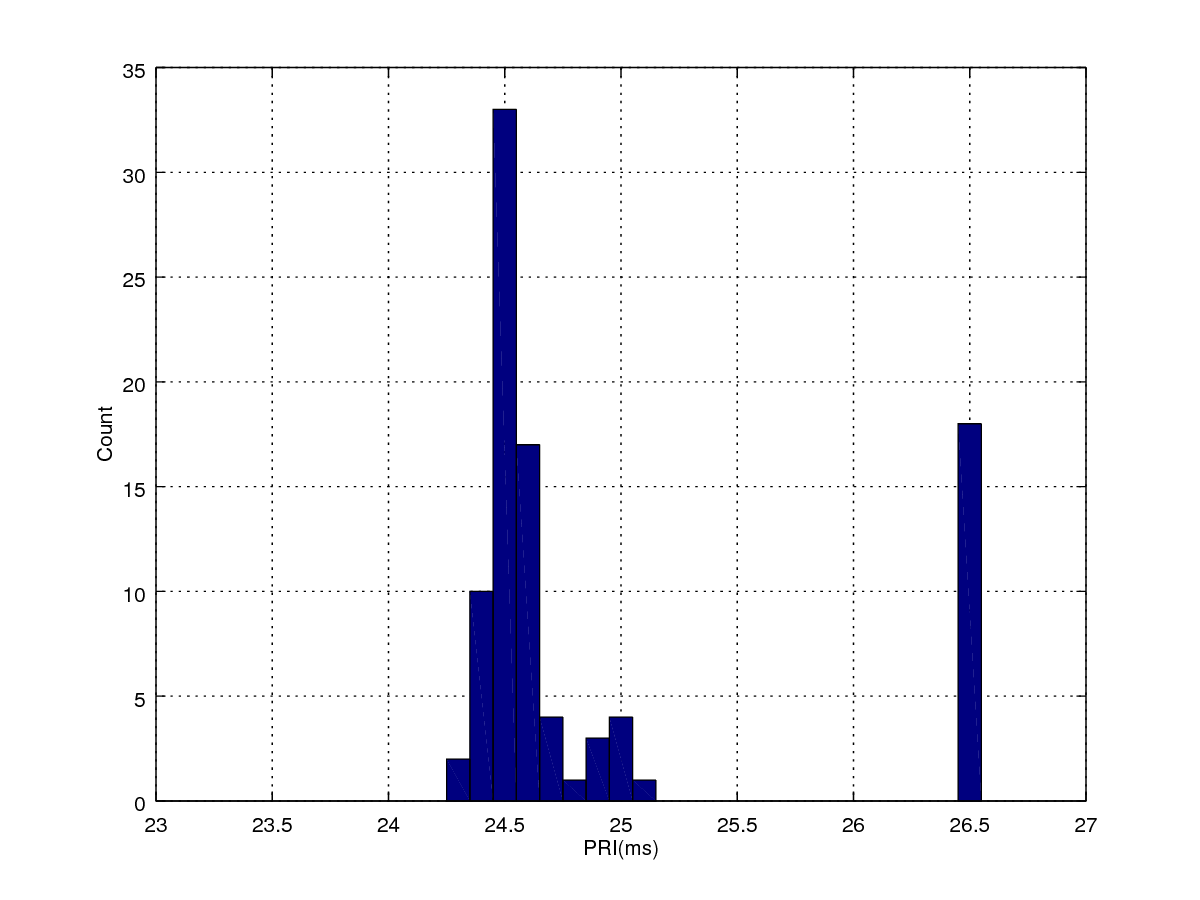
\includegraphics[width=\textwidth]{fig/noncoresec_ping_cc2538_sw.png}
	}
	\end{subfigure}
	\caption{PING Reponse Time for TelosB and CC2538\label{PINGTiming}}
\end{figure}

%Data Analysis